\chapter{Deep Learning}
Le principali tipologie di apprendimento sono:
\begin{itemize}
      \item \textbf{Supervisionato} (Supervised): i dati utilizzati per
            l'apprendimento sono etichettati (label).
      \item \textbf{Non supervisionato} (Unsupervised): i dati utilizzati per
            l'apprendimento non sono etichettati.
\end{itemize}
Inizialmente, le architetture di deep learning sono state composte da
particolari strutture simili agli enconder-decoder chiamate \textbf{autoencoder}
(figura \ref{fig:autoencoder}). Queste strutture sono reti neurali, costruite
con una particolare struttura a clessidra, il cui compito è quello di imparare
come ricostruire l'input.
\begin{figure}[!ht]
      \centering
      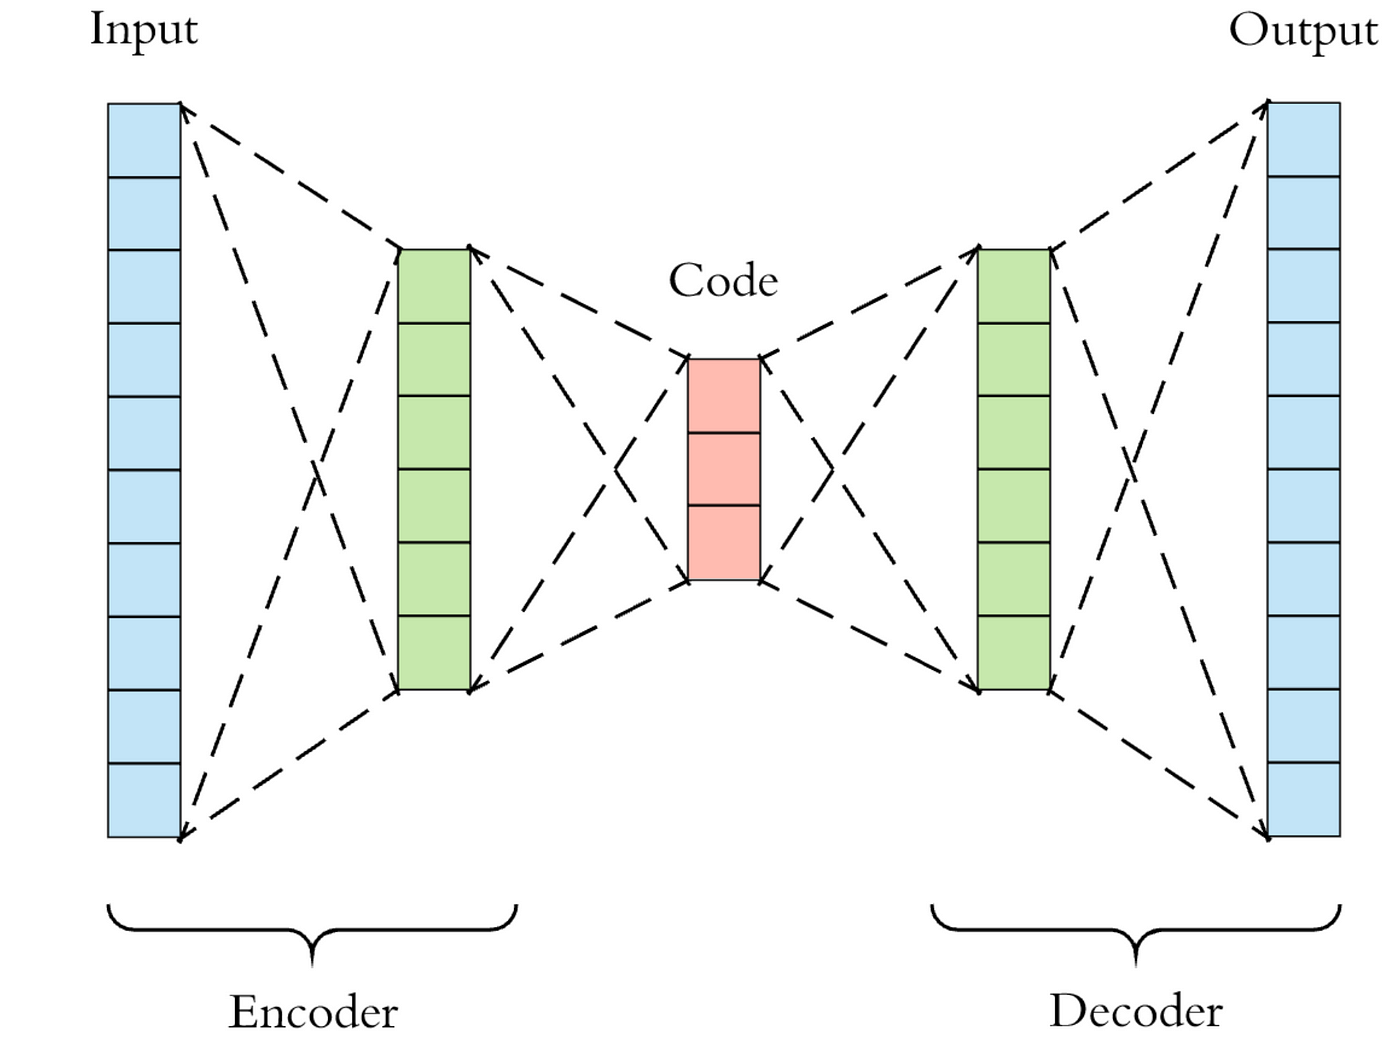
\includegraphics[width=0.5\textwidth]{img/reti/autoencoder.png}
      \caption{Autoencoder}
      \label{fig:autoencoder}
\end{figure}
La metodologia di apprendimento utilizzata dagli autoencoder è unsupervised.
Nella realtà non è del tutto non supervisionata in quanto si ha un \textbf{fake
      task}, ovvero si adotta una metodologia supervisionata in cui non si ha
una label da predire, ma si vuole ottenere l'input stesso. L'obiettivo di
queste reti è quindi quello di ridurre l'errore sulla ricostruzione dell'input.

Il loro risultato è dovuto alla loro struttura, in particolare risulta utile la
codifica ottenuta nel collo di bottiglia che separa la rete in due:
\begin{itemize}
      \item \textbf{Enconder}: impara a codificare l'input utilizzando poche
            informazioni (funzione di codifica, spesso segnata come $Enc(X) = Z$).
      \item \textbf{Deconder}: impara a decodificare l'input partendo da poche
            informazioni (funzione di decodifica, spesso segnata come $Dec(Z) = Y$).
\end{itemize}
L'algoritmo di apprendimento di queste reti spesso è una delle tante
implementazioni di backpropagation, applicandolo su ciascun neurone di uscita.
Più precisamente l'apprendimento si effettua definendo una \textbf{funzione di
      loss} $\mathcal{L}$ che calcolerà la distanza tra l'output del decoder $Y$
e l'input $X$ della rete:
\begin{equation}
      \mathcal{L} = \| X - Y \|
\end{equation}
Per gli autoencoder si deve obbligatoriamente avere sempre una struttura a
clessidra con la strozzatura centrale, la quale permette di generare la codifica
e separare le due reti. In aggiunta, l'architettura non prevede che ci siano
collegamenti tra encoder e decoder altrimenti la codifica nella strozzatura non
sarebbe più consistente.

L'encoder della rete non fa altro che trovare una codifica dell'input in uno
spazio di dimensioni ridotto, questo significa che equivale a calcolare la PCA
sull'input, con la differenza che uno utilizza una rete neurale mentre l'altro
è un processo iterativo basato sugli autovalori e autovettori. Più precisamente
PCA cambia il sistema di riferimento dello spazio in modo tale che gli assi
siano in direzione della massima variabilità. Vista questa dualità con la PCA,
gli autoencoder possono trovare una rappresentazione dell'input a dimensioni
minori per risolvere dei task specifici. La rappresentazione codificata prenderà
il nome di \textbf{rappresentazione latente}.

L'autoencoder può essere utilizzato anche per effettuare task di classificazione
più precisamente si allena l'autoencoder e nel mentre si allena una rete che
prende la rappresentazione latente e la classifica. Quindi la rete sarà formata
da:
\begin{itemize}
      \item Encoder: $Z = Enc_{\theta_1}(X)$
      \item Classificatore: $\hat{y} = F(Z)$
      \item Decoder: $Y = Dec_{\theta_2}(Z)$
\end{itemize}
La loss dovrà essere l'unione delle loss del classificatore e dell'autoencoder.
\begin{equation}
      \mathcal{L} = \| X - Y \| + \| y - \hat{y} \|
\end{equation}

Le architetture odierne di deep learning si basano su strutture neurali e
utilizzano i \textbf{transformer} (figura \ref{fig:transformer}), componenti
neurali che prendono in input sia il nuovo input, sia un vecchio output del
transformer shiftato a destra. Sono componenti fondamentali per la generazione
di informazioni. L'apprendimento di queste reti si basa su strutture \textbf{feed
      -forward} e su componenti \textbf{Attention}, quest'ultimi fondamentali
perché permettono l'effettivo cambiamento dei valori.
\begin{figure}[!ht]
      \centering
      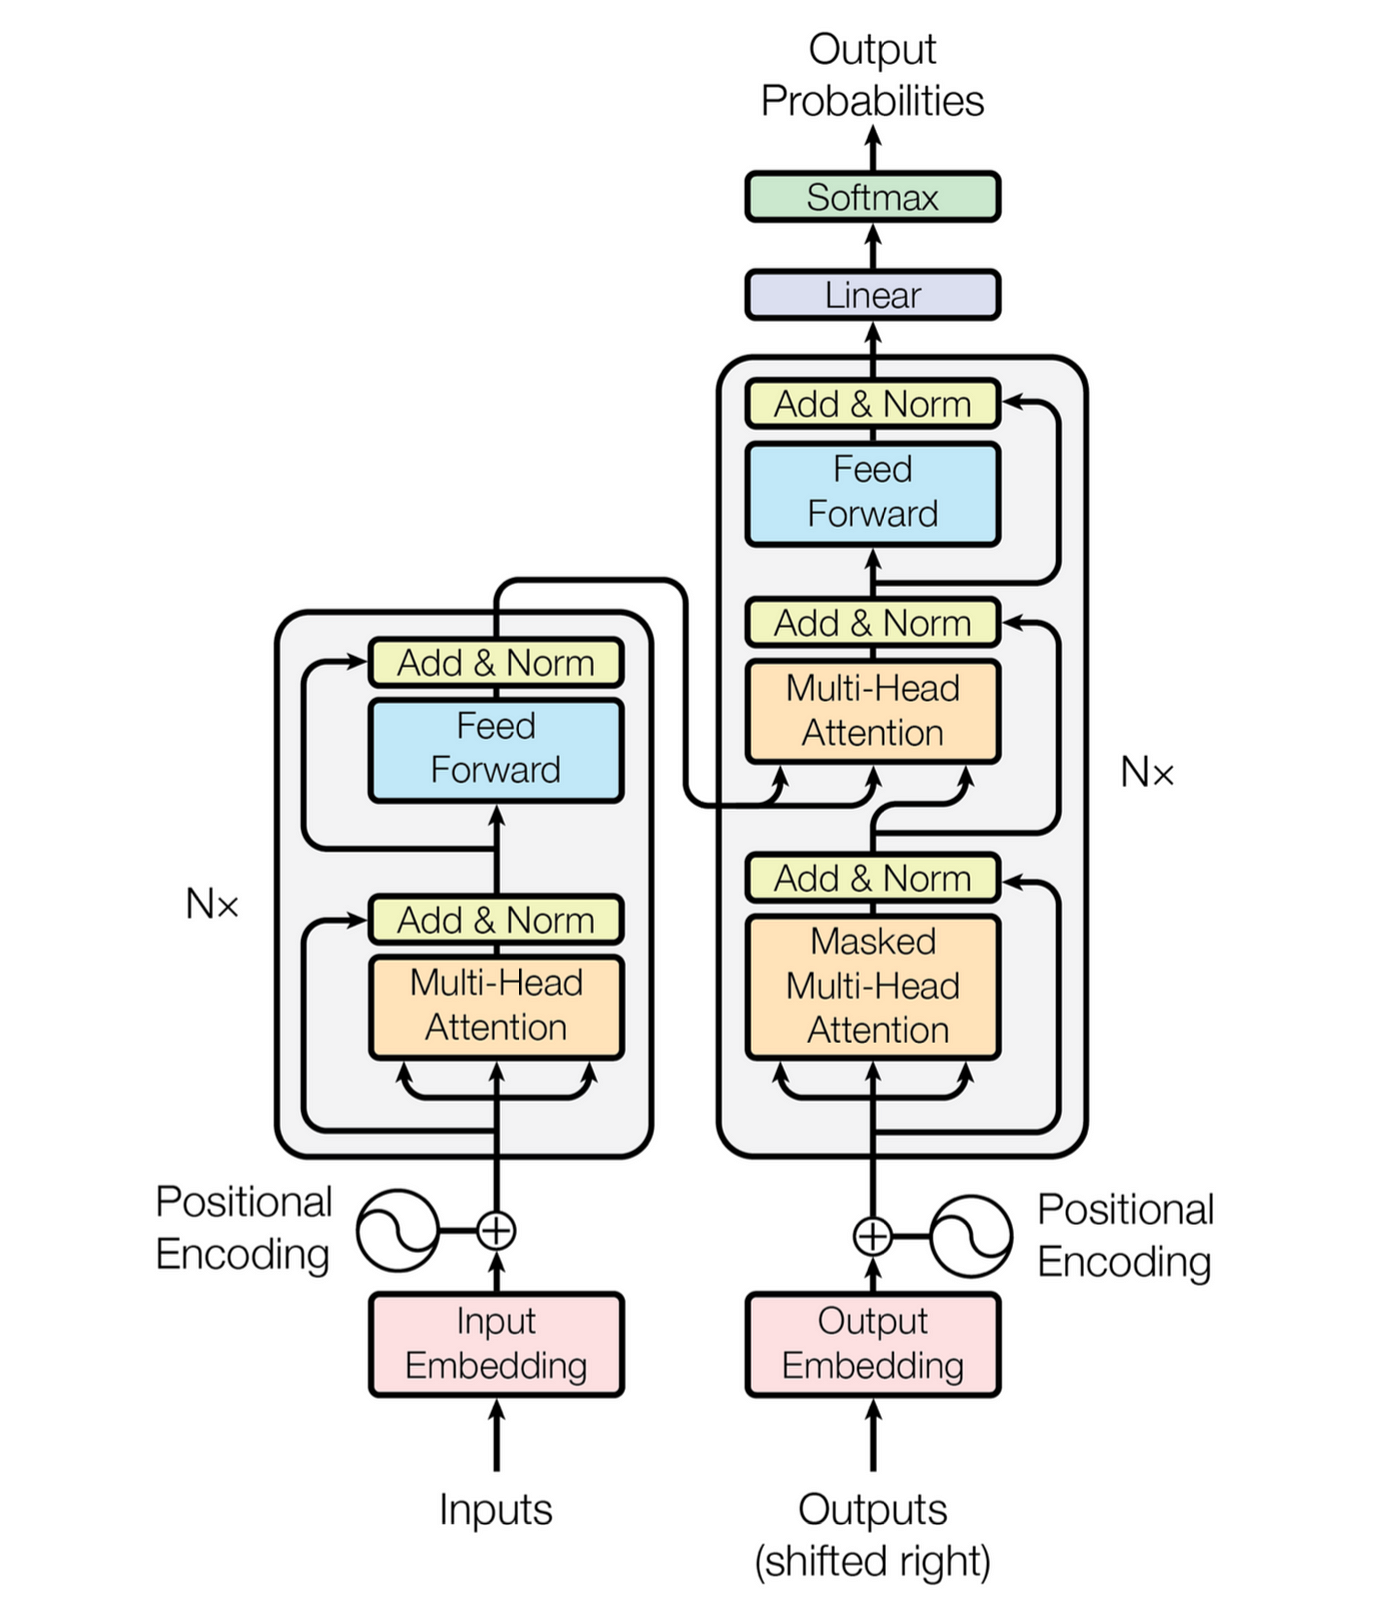
\includegraphics[width=0.5\textwidth]{img/deepl/transformer.png}
      \caption{Struttura di un transformer}
      \label{fig:transformer}
\end{figure}
Prima di arrivare ai transformer si è passati dagli autoencoder, a
\textbf{Word2Vec}, un modello neurale utilizzato per problemi di \textbf{NPL}.
Più precisamente si occupa di associare per ogni parola del linguaggio un vettore
di numeri reali, in questo modo è possibile rappresentare le singole parole in
uno spazio $n$-dimensionale. Questa proprietà ha permesso di scoprire una
proprietà: parole simili vengono rappresentate in una regione vicina dello
spazio. Questo è dato dal fatto che le reti vengono allenate su tutti i testi
raggiungibili e l'assegnamento del vettore si effettua in base a quante volte
due parole vengono veste vicine in una frase. Quindi la rete riesce a codificare
come vettori simili parole simili, infatti c'è una corrispondenza geometrica col
significato.

Successivamente si è passati ai \textbf{denoising autoencoder} (figura
\ref{fig:denoising}), ovvero rimozione del rumore e ricostruzione dell'input
originale. Queste reti vengono allenate dando in input il dato sporcato in
precedenza, successivamente l'output viene confrontato con l'input originale.
\begin{figure}[!ht]
      \centering
      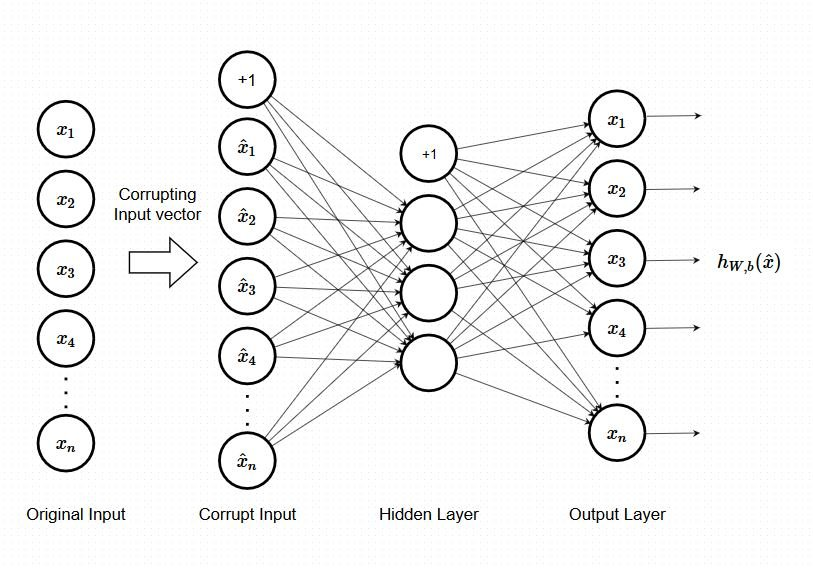
\includegraphics[width=0.5\textwidth]{img/deepl/DenoisingAutoencoder.png}
      \caption{Denoising autoencoder}
      \label{fig:denoising}
\end{figure}
Questa tipologia di rete è nata con lo scopo di impedire all'autoencoder di
imparare la funzione identità, questo perché quando l'autoencoder ha dimensioni
troppo elevate, la rete impara a copiare l'input in output senza effettuare
nessuna trasformazione. Per questo motivo si è deciso di aggiungere del rumore
all'input, in modo da rendere più difficile la ricostruzione dell'input
originale.

In seguito, sono stati introdotti i componenti \textbf{Attention} (figura
\ref{fig:attention}), composti da 3 elementi in input e il suo compito è di
assegnare in automatico diversi pesi agli elementi in input. Queste reti
permettono quindi di cambiare i pesi degli input portando a dei vantaggi notevoli,
per esempio, si possono interpretare parole ambigue in base al contesto.
\begin{figure}[!ht]
      \centering
      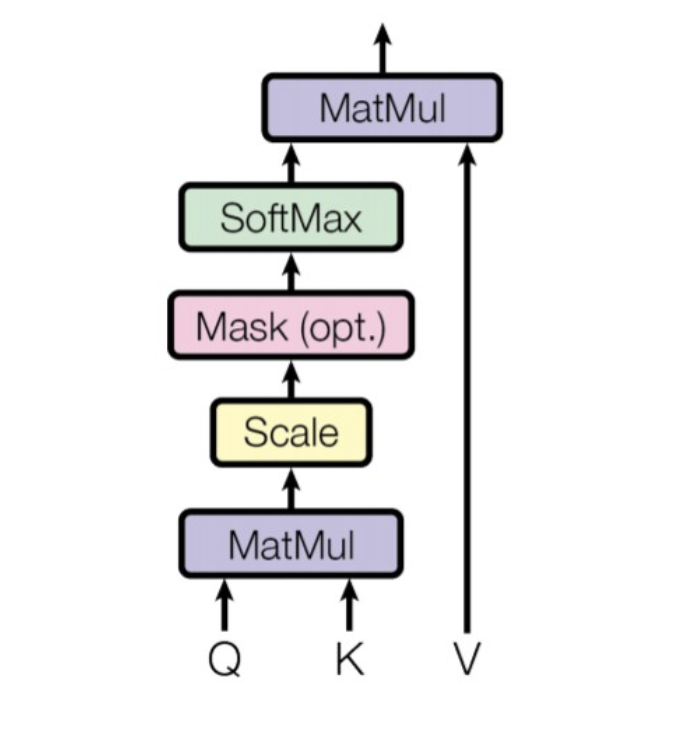
\includegraphics[width=0.5\textwidth]{img/deepl/attention.png}
      \caption{Componente Attention}
      \label{fig:attention}
\end{figure}
Infine, si è passati ai transformer, un modello che evita la ricorrenza e si
basa invece interamente sui meccanismi di attention per valutare le dipendenze
dei dati tra input e output. Utilizzando strutture encoder-decoder, rimuovendo
la ricorrenza in favore dei meccanismi di attention.
%% FONTE: https://paperswithcode.com/method/transformer

I modelli di deep learning vengono allenati in 2 fasi:
\begin{itemize}
      \item \textbf{pre-training generico}: allenamento non supervisionato, si
            allena la rete in modo generale senza specificare un particolare
            task. Questa fase è la più pesante e permette di definire un primo
            stato di partenza dei parametri.
      \item \textbf{fine tuning}: si prende la rete pre-allenata e si addestra
            per un task specifico utilizzando la metodologia supervisionata.
\end{itemize}
In questo modo è possibile ridurre i tempi di addestramento e rendere
riutilizzabile la stessa rete per task simili.

Alla fine si arriva alla creazione di reti più complesse come GPT, basata sempre
su transformer e attention, ma addestrata in 2 fasi, con la possibilità di
effettuare del reinforcement learning per migliorare ancora di più i risultati.